\documentclass[english,submission]{programming}
%% First parameter: the language is 'english'.
%% Second parameter: use 'submission' for initial submission, remove it for camera-ready (see 5.1)


\usepackage[backend=biber]{biblatex}

\usepackage{macros}

\addbibresource{main.bib}

\usepackage{hyperref}
\usepackage[inline]{enumitem} % for inline lists

% this needs to be loaded AFTER hyperref
\usepackage{cleveref}
\usepackage{js}

\begin{document}

\title{Parametric Runtime Verification of Node.js Applications with Trace Expressions}
\subtitle{}% optional
\titlerunning{Parametric Runtime Verification of Node.js Applications with Trace Expressions} %optional, in case that the title is too long; the running title should fit into the top page column

\author{Davide Ancona}
\authorinfo{\email{davide.ancona@unige.it}.}
\author{Luca Franceschini}
\authorinfo{\email{luca.franceschini@dibris.unige.it}.}
\author{Giorgio Delzanno}
\authorinfo{\email{giorgio.delzanno@unige.it}.}
\author{Maurizio Leotta}
\authorinfo{\email{maurizio.leotta@unige.it}.}
\author{Marina Ribaudo}
\authorinfo{\email{marina.ribaudo@unige.it}.}
\author{Filippo Ricca}
\authorinfo{\email{filippo.ricca@unige.it}.}
\affiliation{DIBRIS, University of Genova, Italy}

\authorrunning{D. Ancona, L. Franceschini, G. Delzanno, M. Leotta, M. Ribaudo, F. Ricca} % Optional, for long author lists

\keywords{parametric runtime verification, trace expressions, Jalangi2, Node.js, SWI-Prolog} % please provide 1--5 keywords


%%%%%%%%%%%%%%%%%%
%% These data MUST be filled for your submission. (see 5.3)
\paperdetails{
  %% perspective options are: art, sciencetheoretical, scienceempirical, engineering.
  %% Choose exactly the one that best describes this work. (see 2.1)
  perspective=scienceempirical,
  %% State one or more areas, separated by a comma. (see 2.2)
  %% Please see list of areas in http://programming-journal.org/cfp/
  %% The list is open-ended, so use other areas if yours is/are not listed.
  area={Program verification, testing and debugging},
  %% You may choose the license for your paper (see 3.)
  %% License options include: cc-by (default), cc-by-nc
  % license=cc-by,
}
%%%%%%%%%%%%%%%%%%

%%%%%%%%%%%%%%%%%%
%% These data are provided by the editors. May be left out on submission.
%\paperdetails{
%  submitted=2016-08-10,
%  published=2016-10-11,
%  year=2016,
%  volume=1,
%  issue=1,
%  articlenumber=1,
%}
%%%%%%%%%%%%%%%%%%

%%%%%%%%%%%%%%%%%%%%%%%%%%%%%
% Please go to https://dl.acm.org/ccs/ccs.cfm and generate your Classification
% System [view CCS TeX Code] stanz and copy _all of it_ to this place.
%% From HERE
\begin{CCSXML}
<ccs2012>
<concept>
<concept_id>10002944.10011122.10003459</concept_id>
<concept_desc>General and reference~Computing standards, RFCs and guidelines</concept_desc>
<concept_significance>300</concept_significance>
</concept>
<concept>
<concept_id>10010405.10010476.10010477</concept_id>
<concept_desc>Applied computing~Publishing</concept_desc>
<concept_significance>300</concept_significance>
</concept>
</ccs2012>
\end{CCSXML}

\ccsdesc[300]{General and reference~Computing standards, RFCs and guidelines}
\ccsdesc[500]{Applied computing~Publishing}

% To HERE
%%%%%%%%%%%%%%%%%%%%%%%

\maketitle

% Please always include the abstract.
% The abstract MUST be written according to the directives stated in 
% http://programming-journal.org/submission/
% Failure to adhere to the abstract directives may result in the paper
% being returned to the authors.
\begin{abstract}
Node.js is a runtime framework that gained popularity in the last years as it allows
rapid development of lightweight servers in JavaScript; more recently,
it has been successfully employed to support programming for the Internet of Things.
While the asynchronous, single-thread execution model on which Node.js is based turns out to be an effective way to
efficiently handle big volumes of data and requests, it also makes quite challenging to ensure the correct behavior
of code heavily based on nested callbacks which are executed asynchronously. 
To this aim, runtime verification can be a valuable support to tackle such a complex task, and
to complement other software verification techniques based on static analysis or testing.
Furthermore, runtime verification of Node.js can be fruitfully exploited for ensuring the correctness of Internet of Things systems, a challenge 
which has been barely explored so far. 

Trace expressions have been initially devised as a formalism for runtime verification of protocol-compliance
adopted in widespread multiagent system platforms.
Key features of trace expressions are their support for parametricity, which allows definition of specifications
depending on values that can be known only at runtime when events are traced,
and their independence from a particular language and system, obtained through the notion of event domain and type.

In this work we show how trace expressions can be employed in the context of runtime verification for Node.js applications to specify the expected behavior,
and we present the implementation of a corresponding prototype tool allowing automatic monitoring of the correct use
of the features offered by widespread Node.js libraries, as \lstinline{http}.
The implementation is based on the Jalangi2 framework for JavaScript code instrumentation, required to
dynamically trace events, and on SWI-Prolog for supporting trace expressions and the inference engine for their verification.
The tool offers a simple HTTP interface based on JSON to allow runtime verification of distributed and heterogeneous components.

Preliminary benchmarks with the popular the Node.js http module and the Express framework show that the tool is able to support runtime verification of real Node.js code. 
\end{abstract}

\section{Introduction}
\emph{Node.js} is an increasingly popular runtime environment that supports server-side programming in JavaScript.
At its core, it is based on an asynchronous model of computation: I/O requests are non-blocking and they immediately return to the caller, non-deterministically scheduling the request for later execution.
Furthermore, while I/O operations can be parallelized by the underlying system, the JavaScript code always runs on a single thread.
This asynchronous, single-thread execution model turned out to be an effective way to handle big volumes of data and huge numbers of (simultaneous) requests \cite{Nodejs10,NodejsPerformance14}, thus making Node.js a suitable choice to implement efficient servers without explicitly dealing with multi-threading and parallelism.


%Besides, the huge package ecosystem promotes code reuse and fast development.
%Finally, Node.js recently gained popularity in the Internet of Things community as well.
%
%From a software engineering point of view however, Node.js has its downsides and pitfalls and poses serious challenges.

On the other hand, asynchronous programming heavily relies on the notion of callback, which can lead to many levels of nested blocks and obfuscate the actual execution flow, making the code hard both to read and to debug.
In reaction to an asynchronous request, a callback function is executed on the result of the corresponding operation when available.
This, together with the non-deterministic scheduling of requests, and the dynamic nature of JavaScript itself, are challenges to ensure correct program behavior with traditional approaches like static/formal verification techniques and testing.

\emph{Runtime verification} (RV) \cite{rv} is a software analysis approach in which a running system is observed by monitors that perceive relevant events and use their associated information to verify them against a given formal specification of the expected behavior.
When efficiently implemented, it can even support post production release verification.

As preliminary results suggest \cite{TowardsIoT17}, RV can be fruitfully used to monitor Node.js systems as a complement to formal verification and testing.
The approach suggested in \cite{TowardsIoT17} to implement a monitoring system for JavaScript and Node.js is based on code instrumentation, to allow suitable (and automatic) modification of the original code for appropriate reaction upon occurrences of interesting events.

For specifying systems behavior we use \emph{trace expressions} \cite{ancona2016comparing}, a formalism which is more expressive than others
commonly adopted for RV, as
attributed context-free grammars \cite{de2014combining} and LTL\textsubscript{3} \cite{ltl3}; see \cite{AnconaFM16} for a comparison between trace expressions and linear temporal logics.

Though trace expressions were initially devised to verify protocol-compliance in multi-agent systems, more recently they have been successfully
used as a more general specification formalism \cite{ParametricJava17, TowardsIoT17} thanks to their independence from the monitored system and underlying programming language, obtained through the abstraction of event type;
furthermore, they support \emph{parametric} verification, a key feature to increase the expressive power of the formalism and, hence, allow RV of complex properties whose specification may depend on the actual values associated with events at runtime.

In this work we show how trace expressions can be successfully used to support RV of Node.js applications, a topic that has not
been fully investigated yet;  to this aim, from the documentation of Node.js we have mined the main constraints that have
to be met to correctly use the functions exported by a module, and translated into trace expressions to allow RV of
such constraints.

A corresponding prototype%
%\footnote{The implementation and a script for running all tests reported in this paper are available at \url{https://github.com/LucaFranceschini/trace-expressions}.}
\footnote{Implementations and test at \url{https://github.com/LucaFranceschini/trace-expressions}.}
has been developed based on the Jalangi2\footnote{\url{https://github.com/Samsung/jalangi2}.}
framework and SWI-Prolog\footnote{\url{http://www.swi-prolog.org}.}.
The former is employed for instrumentation of JavaScript code, to be able
to dynamically trace all those events that constitute what we call an \emph{event domain}, that is, the set
of all events relevant to certain kinds of properties;
all examples shown in this paper refer to a unique event domain consisting of calls and returns
from asynchronous functions and their corresponding callbacks. Hence, a unique instrumentation
was required to automatically monitor and verify different properties, each specified by a particular trace expression.
SWI-Prolog is the underlying language for supporting parametric
trace expressions and implementing the inference engine for their verification.

The tool offers a simple HTTP interface based on JSON to allow RV of
distributed and heterogeneous components.
%; in this way, the tool is ready to support RV in the context of the Internet of Things.
%
To test the tool, we have inspected the documentation of the standard \lstinline{http} module, one of the most frequently used
in Node.js, to mine specifications expressible with trace expressions, with the aim of dynamically verifying
the correct use of \lstinline{http} in Node.js code.
Preliminary tests with Express, one of the most popular framework for web applications built on \lstinline{http}, show
that our prototype tool is able to support RV of real Node.js code.

The novel contributions w.r.t. our previous work \cite{TowardsIoT17} can be summarized as follows:
\begin{enumerate*}[label=(\alph*)]
	\item we present a more complete set of examples, including HTTP interactions and the Express framework;
	\item we enhance our implementation in order to keep track of target objects in method invocations (necessary for monitoring HTTP interactions) and to deal with cyclic objects;
	\item we optimize our system by filtering events that are not relevant for the verified specification to avoid sending useless requests to the monitoring server, and by making the communication between the monitored program and the monitor asynchronous.
          %% to fit the Node.js execution model without suspending the execution of the program every time an event is observed.
	\item we measure our performance with benchmarks.
\end{enumerate*}
%More details can be found in the following subsections.

%\vspace{-.3cm}
\paragraph{Outline}
\Cref{sec:node,sec:rv,sec:trace} give the necessary background and state of the art on Node.js, RV and trace expressions, respectively.
%\Cref{sec:node} motivates the choice of Node.js, and together with \Cref{sec:trace} they give the necessary background about Node.js and trace expressions.
%\Cref{sec:rv} is a study of the state of the art for RV techniques, while
\Cref{sec:examples} shows how the approach can help to detect bugs in Node.js programs with motivating examples.
\Cref{sec:impl} presents the implementation of our framework for RV of Node.js based on trace expressions.
\Cref{sec:exps} reports on some preliminary experiments conducted with Node.js programs based on the standard module
\lstinline{http} and the widely adopted framework Express.
Finally, \Cref{sec:conclu} draws conclusions and discusses future research directions.


\section{Node.js}
\label{sec:node}
\begin{figure}
	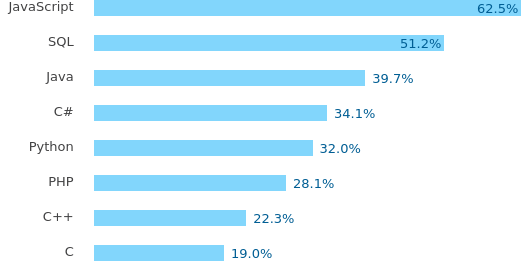
\includegraphics[width=.5\textwidth]{fig/languages}
	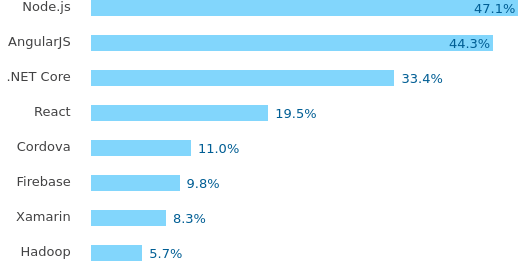
\includegraphics[width=.5\textwidth]{fig/frameworks}
	\caption{Stack Overflow Developer Survey 2017, \url{https://insights.stackoverflow.com/survey/2017}. Most used programming languages (on the left) and frameworks (on the right).}
	\label{fig:popularity}
\end{figure}
%\paragraph{JavaScript}
%According to a survey conducted among developers all over the world by the Stack Overflow website, JavaScript is currently the most popular programming language (\Cref{fig:popularity}), having been a de facto standard for client-side web development for a long time.

%JavaScript is a high-level, dynamic scripting language supporting multiple paradigms: imperative, object-oriented, event-driven and functional programming.
%Standardized as EcmaScript \cite{EcmaScript}, the language is under active development and new features are constantly added, with the latest stable version released in June 2017.

\paragraph{Node.js}
In 2009 Node.js\footnote{\url{https://nodejs.org/}} was released, and since then its popularity quickly raised to the point that it now appears to be the single most used framework, according to Stack Overflow Developer Survey 2017 (\Cref{fig:popularity}).
Node.js is a JavaScript runtime environment expressly devised for running JavaScript code outside web browsers, thus giving developers the opportunity to use the language to write server-side code as well.

Node.js is based on Chrome V8, a highly optimized JavaScript engine developed for the Google Chrome web browser. 
Furthermore, developers can count on a huge package ecosystem\footnote{\url{https://www.npmjs.com/}} with a repository of hundreds of thousand modules that can be reused.
More recently, Node.js has become relevant for the Internet of Things as well, both because of the availability of packages for device management and its asynchronous model, which is well suited for distributed environments.
Node-RED\footnote{\url{https://nodered.org/}} is a tool based on Node.js to support flow-based programming for the Internet of Things to
connect together devices at the edge of the network.

\paragraph{Asynchronous Computation}
%The execution model of Node.js is quite different from most of other environments.
In Node.js, connection to databases, HTTP requests, access to the file system and every other I/O intensive operation is by default \emph{asynchronous}, meaning the actual execution is postponed until a later time, and the program can go on without waiting for completion.
Computations needing the results of I/O operations are modeled by \emph{callbacks}: when an asynchronous function is invoked, another function (the callback) is given as an additional argument, and it will be executed once the results will be available.

\Cref{lst:async} shows the different programming patterns using synchronous and asynchronous calls.
On the left, the program is blocked until the result of \lstinline{syncIO} is returned, and then it is passed to function \lstinline{use}.
On the right, \lstinline{asyncIO} \emph{immediately returns} and the I/O operation is scheduled for execution together with the callback \lstinline{use}; when the result will be available, the callback will be executed receiving such result as an argument.
Node.js heavily takes advantage of the right pattern (for the sake of brevity, error handling is ignored in the example).

\begin{figure}[h]
\begin{minipage}{.5\textwidth}
\begin{lstlisting}
	function use(data) { ... }
	let res = syncIO(...);
	use(res);
\end{lstlisting}
\end{minipage}
\begin{minipage}{.5\textwidth}
	\begin{lstlisting}
	function use(data) { ... }
	asyncIO(..., use);
	\end{lstlisting}
\end{minipage}
\caption{Difference between synchronous and asynchronous I/O.}
\label{lst:async}
\end{figure}

\paragraph{Event Loop}
The core of Node.js is the \emph{event loop}, represented in \Cref{fig:eventloop}.
Asynchronous requests are processed from a simple loop, and the corresponding I/O intensive operations are scheduled for execution together with their callbacks.
The event loop is run after the whole Node.js script is evaluated.

\begin{figure}[h]
	\centering
	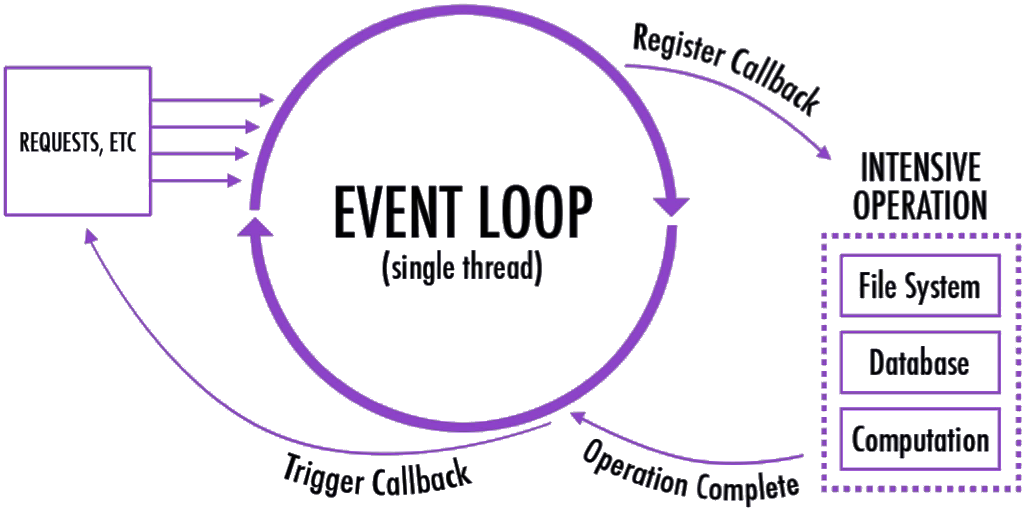
\includegraphics[width=.7\textwidth]{fig/event-loop}
	\caption{Node.js execution model representation based on the event loop.}
	\label{fig:eventloop}
\end{figure}

Note that callbacks themselves can make more asynchronous requests to the event loop, and those requests will receive callbacks, and so on\dots{}
Indeed, in real programs callbacks and I/O operations are usually nested into each other as a synchronization mechanism, making it hard to understand (and debug) the code.

Even if it may seem counterintuitive at first, this execution model based on asynchronous I/O and the event loop scales very well to a lot of concurrent operations, without the need for the programmer to explicitly deal with concurrency and parallelism \cite{Nodejs10,NodejsPerformance14}.
At the system level, different I/O operations can be executed in parallel.


\section{Runtime Verification}
\label{sec:rv}
\paragraph{Context}
Historically, different approaches has been proposed to solve the problem of verifying the behavior of software systems.

On one hand \emph{formal methods} has been proposed, including theorem proving \cite{itp}, a semi-automated class of techniques inspired by mathematical proofs, and model checking \cite{modelchecking}, which aims to automatically verify a suitably small model of the system against expected properties.
These techniques have been extensively studied in the literature and are quite mature.
However, they require either a deep theoretical knowledge or a simplified model of the system, and this may not be the case for many real-world scenarios.

On the other hand, software \emph{testing} \cite{testing} has been successfully employed in industry, to find bugs by running (part of) the system on input whose correct output is known.
Testing proved itself useful by working on many different levels of abstraction, from unit-test of small code snippets to black-box testing of complex systems as a whole.

More recently another approach to the problem has been proposed, that is, \emph{Runtime Verification} \cite{rv}.
%as suggested by the name, consists in verifying a real run of the system against a given specification.
First, a \emph{monitor} is attached to the system under test in order to observe all relevant events.
The result of this is said to be a \emph{trace}, and it encodes the observed run.
Then, the trace is verified against correctness properties expressed in a suitable formalism.

\paragraph{Word Problem}
Runtime verification is often considered a \emph{lightweight} verification technique, since it aims at analyzing only a \emph{single run} of the system, and not all the possible execution paths (as it is customary, for instance, in model checking).
If we think of correctness properties as some set \(S\) of traces satisfying them, the problem tackled by runtime verification is clearly easier than the one solved by static techniques.
Essentially it is a \emph{word problem} (check whether a given trace belongs to \(S\)) rather than an \emph{inclusion} problem (check whether the set of all possible traces is included in \(S\)).

%TODO: c'\`e un esempio nel survey di Leucker sugli NDFA volendo: l'inclusione fra NDFA \`e PSPACE-completa ma l'appartenenza \`e NL-completa (non deterministico logaritmica), e l'inclusione fra le due classi \`e stretta. Forse per\`o \`e un po' ``hardcore''...

\paragraph{Expressiveness}
Part of the complexity comes from the expressiveness of the specification language in use, and different formalisms have been proposed,
including regular expressions, context-free grammars with attributes \cite{de2014combining,BoerEtAl14},
and \emph{Linear Temporal Logic (LTL)} \cite{ltl} (and its variations), a modal logic where modalities refer to time which is
one of the most commonly used specification formalism. 
While LTL deals with infinite traces, when doing runtime verification traces are always finite for obvious reasons.
Nonetheless, it is useful to verify non-terminating systems: in such cases, only finite trace prefixes are available.
In order to deal with this, \emph{LTL\textsubscript{3}} has been proposed as a three-valued LTL \cite{ltl3}, with the additional truth value encoding an inconclusive verification result.

%The formalism we plan (and already started) to use, i.e., \emph{trace expressions} \cite{AnconaDM12, AnconaBB0CDGGGH16}, compares well to linear temporal logics.
Though they are not comparable to LTL (meaning none of them is more expressive than the other), trace expressions \emph{are} more expressive than LTL\textsubscript{3} \cite{ancona2016comparing}, which is very relevant for runtime verification purposes since the formalism has explicitly been devised for that \cite{ltl3}.

\paragraph{Monitoring Techniques}
Besides specification, a crucial point of runtime verification is the monitoring part, which can either be \emph{offline} or \emph{online}.
With the former approach, the execution is observed and, in the end, a trace is produced as a result; then it is checked against the specification.
The latter approach can offer more possibilities, since events are observed by the monitor as soon as they occur, and the updated trace is checked in real-time.
While this can slow down the execution, it offers some advantages.
Not only errors are caught (almost) as soon as they manifest, but it is also possible to take \emph{recovery actions} \cite{ancona2015global} in case
monitoring is efficient enough to be performed even after deployment.

Programs implementing such behaviors have to be aware of the monitor and to interact with it.
Different patterns and paradigms have been proposed for this, see \emph{Monitor-Oriented Programming (MOP)} \cite{mop}, a framework for runtime verification of Java programs, or \emph{Runtime Reflection} \cite{rr}, an architectural pattern designed for monitor-aware systems able to diagnose problems and mitigate issues.

Another critical aspect of runtime verification systems is the generation of the monitor itself, especially since it is desirable to automatically generate them from the high-level formal specification, thus making their adoption and application easier.
Such a monitor should avoid to interfere with the program behavior as much as possible, in order for the verification to be effective.
This is very important when the system under test has to operate in real-time, and/or when the property to be checked contains time constraints itself.

\paragraph{Applications}
Runtime verification can also be seen as a complement to more traditional approaches, like formal methods and testing, either for inherently dynamic properties that otherwise would be hard to verify, or for (safety-)critical systems that needs to be constantly checked, even \emph{after deployment} and not only during the development cycle.
Runtime verification can be used in conjunction with testing in order to generate test cases, as shown in \cite{artho2005combining}.
As a note, however, neither testing nor runtime verification are \emph{complete}.
In other words, they cannot prove that a program satisfy some property for every input.

Runtime verification has been successfully applied to many other contexts, including \emph{web services and applications} \cite{webservices, webapps}, \emph{multi-agent systems} \cite{AnconaDM12}, \emph{object-oriented languages} \cite{pql, javadynamic, de2014combining, BoerEtAl14} and the \emph{Internet of Things} \cite{rviot1, rviot2}.

\paragraph{Node.js}
In the context of runtime verification, we only found one work that has been applied to Node.js applications \cite{Rosenberg2016}.
The approach is based on DTrace \cite{dtrace}, a low-level dynamic tracing framework that allows to extract a trace from a running system.
However, there are important differences both in the implementation and in the goals.
The monitors produces in the cited work exploit LTL \cite{ltl} as a specification formalism, thus parametric verification is not supported, but as we show in the examples this is an important feature that increases expressiveness.
Moreover, since one of our goals is to target the Internet of Things, we chose a distributed approach with a remote monitoring server.
On the other hand, DTrace is not distributed and works at a lower level, thus being more efficient.

\paragraph*{}
For a more in-depth, authoritative survey of runtime verification see \cite{rv}.


\section{Trace Expressions}
\label{sec:trace}
Trace expressions were initially developed in the context of multi-agent systems as ``global types'' \cite{AnconaDM12}.
The aim was to obtain a formalism expressive enough to check messages exchanged by autonomous agents for compliance against a given interaction protocol \cite{AnconaBFMT14, BriolaMA14}.
Global types, and thus trace expressions, derive from the notion of behavioral type, for which a survey can be found in \cite{AnconaBB0CDGGGH16}.

Later on, with the introduction of the notion of event type, trace expressions have become system and language agnostic, so that they can be exploited for runtime verification in several different contexts.

We chose trace expressions as a specification formalism for different reasons: they are quite expressive \cite{ancona2016comparing}, they support parametricity \cite{AnconaFM17} and they can be directly implemented in Prolog (see \cite{TowardsIoT17} for more information on the implementation of a monitoring system based on trace expressions).
Furthermore they are syntactically regular terms \cite{Courcelle83}, which makes it natural to express recursion and (possibly) non-terminating system, and easy to write them as cyclic terms in Prolog.
Trace expressions differs from type-based approaches, as session types \cite{sessiontypes}, in their focus on runtime verification rather than static checking, as their goal is to allow efficient online monitoring.
Just like trace expressions specify the behaviour of the program as a whole, global session types have been proposed as well \cite{globalst,Vasconcelos11}.
A more thorough comparison between these two different approaches is left to future work.

\paragraph{Events}
Trace expressions can be used to specify the possible correct behavior of a system, w.r.t.\ some property that needs to be verified.
To this aim, \emph{events} are defined as all the relevant observations that can be made on the system.
Examples include the execution of I/O operations, the triggering of a Node.js callback, invocation of functions\textellipsis{} A fixed set \(\eventSet\) of events is assumed.

An \emph{event trace} \(\ev_1\dots \ev_n\dots\) is a (possibly infinite) sequence of events.
Using formal language notation, the set of traces can be denoted as \(\eventSet^\infty = \eventSet^* \cup \eventSet^\omega\) (the union of all finite and infinite traces, respectively).
Intuitively a trace encodes a run of the system under test, or at least the relevant parts of its execution.

As an example, consider the monitoring of a program writing on files.
The set of relevant events could be, for instance, the three common operations \emph{open}, \emph{write} and \emph{close}, where \(\fd\) is the unique file descriptor:
%\[\mathcal{E} = \{ \mathit{open}(\mathit{fd}) \mid \mathit{fd} \in \mathbb{N} \} \cup
%\{ \mathit{write}(\mathit{fd}) \mid \mathit{fd} \in \mathbb{N} \} \cup
%\{ \mathit{close}(\mathit{fd}) \mid \mathit{fd} \in \mathbb{N} \} \]
\begin{equation}\label{eq:filedomain}
\eventSet = \bigcup_{\fd \in \mathbb{N}} \{\opent(\fd), \writet(\fd), \closet(\fd)\}
\end{equation}

An example of event trace over the set \(\eventSet\) would be the following:
\begin{equation} \label{eq:trace}
	\opent(42)\ \writet(42)\ \writet(42)\ \closet(42)
\end{equation}

\paragraph{Event Types}
On the top of events, a language \(\eventTySet\) of \emph{event types} is defined.
Event types are generally terms allowed to contain variables, and their language is not fixed in order to make trace expressions more flexible and easily adaptable to different domains.

Together with event types a function \(\mtch\) is assumed to be given, with the following semantics.
Given an event \(\ev\) and an event type \(\eventTy\), \(\mtch(\ev, \eventTy) = \subs\) if and only if \(\ev\) matches \(\eventTy\) with the computed substitution \(\subs\); substitutions on terms have the usual meaning.

In the rest of the paper, we consider different examples of event domains and, thus, event type languages.
We do not expect considerable expressivity is needed in this step, and as long as matching and substitution functions are defined, all properties still hold.
Since we will use standard inductive terms over some (implicitly given) signature and a (enumerable) set of variables, the usual definition of substitution apply.

Considering again the previous files event domain (\ref{eq:filedomain}), a sensible event type matching all write operations would be \(\writet(\xv)\), where \(\xv\) is a variable.
A sensible definition of matching would lead to the following:
\[ \mtch(\writet(42), \writet(\xv)) = \{ \xv \mapsto 42 \} \]

%%Trace expressions have been extended with variables in \cite{AnconaFM17}.

\paragraph{Trace Expressions}
Finally, a \emph{trace expression} identifies a set of traces corresponding to correct system behaviors. It is built on top of event types and the following operators:
\begin{itemize}
	\item $\emptyseq$ (\emph{empty trace}): the singleton set $\{\emptyseq\}$ containing  the empty event trace $\emptyseq$;
	\item $\eventTy\prefixop\tau$ (\emph{prefix}): the set of all traces whose first event $\ev$ matches the event type $\eventTy$, and the remaining part is a trace of $\tau$;
	\item $\tau_1\catop\tau_2$ (\emph{concatenation}): the set of all traces obtained by concatenating the traces of $\tau_1$ with those of $\tau_2$; 
	\item $\tau_1\andop \tau_2$ (\emph{intersection}): the intersection of the traces of $\tau_1$ and $\tau_2$;
	\item $\tau_1\orop \tau_2$ (\emph{union}): the union of the traces of $\tau_1$ and $\tau_2$; 
	\item $\tau_1\shuffleop \tau_2$ (\emph{shuffle}, a.k.a. \emph{interleaving}): the set obtained by shuffling the traces of $\tau_1$ with the traces of $\tau_2$;
	\item $\var{x}{\tau}$ (\emph{binder}): it binds the free occurrences of $\xv$ in $\tau$;
	\item $\eventTy\filterop\tau$ (\emph{filter}):
	denoting the set of all traces contained in $\tau$, when they are deprived af all events that do not match $\eventTy$ (theoretically, this operator can also be derived from the others).
\end{itemize}

Trace expressions are regular terms (a.k.a. cyclic) \cite{Courcelle83}, thus there is no need for an explicit recursion operator.

For instance, the following trace expression \(\tau\) specifies the correct use of the file descriptor \(42\):
\begin{align*}
	\tau &= \emptyseq \orop (\opent(42) \prefixop \tau')\\
	\tau' &= (\writet(42) \prefixop \tau') \orop (\closet(42) \prefixop \emptyseq)
\end{align*}
In the first line, \(\opent\) is forced to be the first operation, if any.
After that, in \(\tau'\), either there will be write operations or the file will be closed and no more writes will be allowed.

%% Not all operators will be used in this document, but they all can be useful in different contexts.
%% See \cite{ancona2016comparing} for a complete technical presentation of trace expressions with more examples. 

\paragraph{Parametric Trace Expressions}
The trace expression above can only verify the correct use of a single file descriptor, but with variables and binders \cite{AnconaFM17} it is possible to write a \emph{parametric} specification that solves the problem for any number of files:
\begin{align}
\label{eq:files1}
\tau &= \emptyseq \orop \var{fd}{\opent(\avar{fd}) \prefixop (\tau \shuffleop \tau')}\\
\label{eq:files2}
\tau' &= (\writet(\avar{fd}) \prefixop \tau') \orop (\closet(\avar{fd}) \prefixop \emptyseq)
\end{align}
When the first event \(\opent(x)\) will occur, it will match the prefix computing the substitution \(\{\avar{fd}\mapsto x\}\).
At this point the shuffle operator is crucial:
%\footnote{In order for the shuffle to work, we assume that every \(\opent\) operation always gives a fresh file descriptor, which can be reasonably assumed to be ensured by the operating system.}
following events are allowed to belong either to \(\tau\) (operations on new files, in the correct order) or to \(\tau'\{\avar{fd}\mapsto x\}\) (note the substitution!) where further operations on \(x\) will be checked.

Note that we are not monitoring the correct behavior of the underlying operating system, namely, that the same file descriptor is not assigned to many opened files simultaneously.
Rather, the specification ensures that the API offered by such system is correctly used.

\paragraph{Operational Semantics}
\begin{figure}[t]
\begin{gather*}
%%%% implicit substitution version, local substitution (i.e. substitution is output only)
\Rule{main}
{\tau\extrans{\ev}\tau';\emptyset}
{\tau\trans{\ev}\tau'}
{}
\qquad
\Rule{prefix}
{}
{\eventTy\prefixop\tau\extrans{\ev}\tau;\subs}
{
  \subs=\mtch(\ev,\eventTy)
}
\qquad
\Rule{and}
{\tau_1\extrans{\ev}\tau'_1;\subs_1\quad\tau_2\extrans{\ev}\tau'_2;\subs_2}
{\tau_1\andop\tau_2\extrans{\ev}\tau'_1\andop\tau'_2;\subs}
{\subs=\subs_1\subsMerge\subs_2}
\\[1ex]
\Rule{or-l}
{\tau_1\extrans{\ev}\tau'_1;\subs}
{\tau_1\orop\tau_2\extrans{\ev}\tau'_1;\subs}
{}
\qquad
\Rule{or-r}
{\tau_2\extrans{\ev}\tau'_2;\subs}
{\tau_1\orop\tau_2\extrans{\ev}\tau'_2;\subs}
{}
\qquad
\Rule{shuffle-l}
{\tau_1\extrans{\ev}\tau'_1;\subs}
{\tau_1\shuffleop\tau_2\extrans{\ev}\tau'_1\shuffleop\tau_2;\subs}
{}
\\[1ex]
\Rule{cat-l}
{\tau_1\extrans{\ev}\tau'_1;\subs}
{\tau_1\catop\tau_2\extrans{\ev}\tau'_1\catop\tau_2;\subs}
{}
\qquad
\Rule{cat-r}
{\tau_2\extrans{\ev}\tau'_2;\subs}
{\tau_1\catop\tau_2\extrans{\ev}\tau'_2;\subs}
{\isEmpty(\tau_1)}
\qquad
\Rule{shuffle-r}
{\tau_2\extrans{\ev}\tau'_2;\subs}
{\tau_1\shuffleop\tau_2\extrans{\ev}\tau_1\shuffleop\tau'_2;\subs}
{}
\\[1ex]
\Rule{var-t}
{\tau\extrans{\ev}\tau';\subs}
{\var{\xv}{\tau}\extrans{\ev}\subs\tau';\restrict{\subs}{\xv}}
{\xv\in\dom(\subs)}
\qquad
\Rule{var-f}
{\tau\extrans{\ev}\tau';\subs}
{\var{\xv}{\tau}\extrans{\ev}\var{\xv}{\tau'};\subs}
{\xv\not\in\dom(\subs)}
\\[1ex]
\Rule{filter-t}
{\tau\extrans{\ev}\tau';\subs}
{\eventTy \filterop \tau \extrans{\ev} \eventTy \filterop \tau';\subs}
{\subs=\mtch(\ev,\eventTy)}
\qquad
\Rule{filter-f}
{}
{\eventTy \filterop \tau \extrans{\ev} \eventTy \filterop \tau}
{\not\exists\subs=\mtch(\ev,\eventTy)}
\\[1ex]
\Rule{$\isEmpty$-empty}
{}
{\isEmpty(\emptyseq)}
{}
\qquad
\Rule{$\isEmpty$-var}
{\isEmpty(\tau)}
{\isEmpty(\var{\xv}{\tau})}
{}
\\[1ex]
\Rule{$\isEmpty$-or-l}
{\isEmpty(\tau_1)}
{\isEmpty(\tau_1\orop\tau_2)}
{}
\qquad
\Rule{$\isEmpty$-or-r}
{\isEmpty(\tau_2)}
{\isEmpty(\tau_1\orop\tau_2)}
{}
\qquad
\Rule{$\isEmpty$-others}
{\isEmpty(\tau_1)\quad\isEmpty(\tau_2)}
{\isEmpty(\tau_1 \op\ \tau_2)}
{\op\in\{\shuffleop,\catop,\andop\}}
\end{gather*}

\caption{Transition system for parametric trace expressions.}
\label{fig:semantics}
\end{figure}
The semantics of trace expressions is given by the labeled transition system in \Cref{fig:semantics}.
\( \tau \extrans{\ev} \tau';\subs \) holds iff the trace expression \(\tau\) accepts the event \(\ev\) with the substitution \(\subs\) and rewrites to \(\tau'\).
For instance, considering again trace expressions in \Cref{eq:files1,eq:files2}, the following transition is valid:
%%\[ \tau \extrans{\opent(1)} \tau';\{\avar{fd} \mapsto 1\} \]
\[
  \tau \trans{\opent(1)} \tau\shuffleop \tau'' \quad \mbox{ with }
  \tau''= (\writet(1) \prefixop \tau'') \orop (\closet(1) \prefixop \emptyseq)
\]

Transition rules depend on predicate \(\isEmpty(-)\) which checks for termination, i.e., \(\isEmpty(\tau)\) holds only if \(\tau\) accepts the empty trace \(\emptyseq\).
More generally, a trace expression \(\tau\) accepts a (possibly infinite) event trace \(\ev_1\ev_2\dots\) iff there exists a (possibly infinite) reduction \(\tau \trans{\ev_1} \tau' \trans{\ev_2} \dotsb\).

The operational semantics rule for the intersection operator depends on the side condition \(\subs=\subs_1\subsMerge\subs_2\).
Such equality holds when \(\subs_1\) and \(\subs_2\) coincide on \(\dom(\subs_1) \cap \dom(\subs_2)\).

The top-level rule (main) expects the computed substitution to be empty.
This corresponds to the fact that valid trace expressions, when considered as a whole, are supposed not to have free variables.
However, when a variable is introduced by a binder, it will be substituted in the trace expression (rule (var-t)), and removed from the computed substitution.
Finally, (var-f) handles the case in which a parametric trace expression accepts an event but the matching does not instantiate a variable (for instance, because its value will only be discovered observing further events).

Trace expressions semantics has been implemented in SWI-Prolog.
The logic programming paradigm is well suited for the implementation of inference system, since inference rules can be translated almost directly to logic clauses.
Furthermore SWI-Prolog offers native support to cyclic terms, therefore recursive trace expressions can be easily encoded.
Support for programming with cyclic terms is based on coinductive logic programming \cite{CoLP06}, which is supported by the SWI-Prolog library \texttt{coinduction}.


\section{Monitoring Examples}
\label{sec:examples}
\subsection{Web Request Finalization}
The \lstinline{http} Node.js module exposes a complete API for HTTP clients and servers, and its typical uses are good examples of code that would benefit from runtime verification techniques.

Consider the snippet in \Cref{lst:end}: a HTTP server is created, and the given callback \lstinline|(req, res) => { ... }| defines its behavior, namely, it replies to every request with a response code \lstinline{200} and the content \lstinline{'okay'}.
The anonymous function will be invoked everytime a request is received from a client.

\begin{figure}[h]
\begin{lstlisting}
const http = require('http');
const server = http.createServer((req, res) => {
  res.writeHead(200);
  res.write('okay');
}); // res.end() call missing
server.listen(80);
\end{lstlisting}
\caption{An example of \emph{incorrect} usage of the Node.js \lstinline{http} module.}
\label{lst:end}
\end{figure}

It is possible for the server to send multiple chunks of data calling \lstinline{write}.
After that, the documentation \emph{requires} the programmer to call method \lstinline{end} to finalize the response.
The code above, however, fails to do that, making the client stuck waiting for the end of the response.
This constraint is not enforced by the library itself, and thus developers have to remember to call the \lstinline{end} method.

Trace expressions can be used to formally specify (and later verify) the requirement.
Consider for instance the following event domain:
\[ \eventSet = \bigcup_{\idcb,\idres \in \mathbb{N}} \{\createt(\idcb), \cbt(\idcb, \idres), \writet(\idres), \myend(\idres) \} \]

The four events above encodes calls to \lstinline{http.createServer}, the callback, \lstinline{res.write} and \lstinline{res.end}, respectively.
Every relevant objects has an associated unique identifier, both the callbacks and the response objects: this is needed in order to correctly match them.

We define event types to be event terms over a set of variables \vars used as placeholders for request identifiers (the match will simply compute the appropriate substitution):
\[ \vars = \{ \avar{id_1}, \avar{id_2}, \dotsc \}\qquad
\mathcal{ET} = \bigcup_{\xv,\xv' \in \vars} \{\createt(\xv), \cbt(\xv, \xv'), \writet(\xv), \myend(\xv) \} \]

Finally, the parametric trace expressions formalizing the expected trace of events follows:
\begin{gather*}
	\tau = \var{\idcb{}}{\createt(\idcb{}) \prefixop \tau_{cb}} \qquad\qquad
	\tau_{cb} = \var{\idres{}}{\cbt(\idcb, \idres) \prefixop (\tau_w \shuffleop \tau_{cb})}\\
	\tau_w = (\writet(\idres) \prefixop \tau_w) \orop (\myend(\idres) \prefixop \epsilon)
\end{gather*}

The trace must start with a \(\createt\) event, which also allows to store the identity of the the callback.
Then, once the callback is actually invoked, the identifier of the response object is known and it can later be used to match against subsequent \lstinline|write| and \lstinline|end| calls.

The use of the shuffle operator is crucial: it allows different requests to be handled concurrently, as this can happen when asynchronous computation is performed.

\subsection{Web Requests Length}
\label{sec:web-req}
%Recalling the web server presented in \Cref{lst:http},
Let us consider the (buggy) web client in \Cref{lst:client}, where seven bytes of data are sent (\lstinline{'hey!'}, \lstinline{'bye'}) but ten are declared in the \lstinline{'content-length'} field.
\lstinline{http.request} is an asynchronous operation that schedules the callback \lstinline!res => { ... }! for execution upon receivement of response.
Such callback will simply print the content of the message.

\begin{figure}[h]
\begin{lstlisting}
const http = require('http');
const options = {
	method: 'POST',
	headers: { 'content-length': 10 } };  // BUG! size too high
const req = http.request(options, res => res.on('data', console.log));
req.write('hey!');
req.end('bye');
\end{lstlisting}
\caption{An \emph{incorrect} web client sending a request with the wrong \texttt{content-length} value.}
\label{lst:client}
\end{figure}

The logging callback (\lstinline{console.log}) is scheduled for execution after receiving the response from the server.
However, it will not be called since the server will be waiting for more data, and no reply will be sent.

The \lstinline{'content-length'} is \emph{not} checked by the Node.js runtime against the actual length of the content, as it is clearly stated in the documentation.
Trace expressions can be used again to specify the correct behavior.
The monitor needs to observe the creation of the \lstinline{ClientRequest} object returned by function \lstinline{http.request} as well as the use of its methods \lstinline{write} and \lstinline{end}.

Consider for instance the following event domain:
\[ \eventSet = \bigcup_{\substack{\avar{data} \in \mathbb{B}^* \\ \avar{cl},\id \in \mathbb{N}}} \{ \req(\id,\avar{cl}), \writet(\id, \avar{data}), \myend(\id, \avar{data}) \} \]
All operations are associated with a unique request identifier (at the Node.js level, this corresponds to the \lstinline{ClientRequest} object), furthermore the request is associated with the declared \lstinline{'content-length'} \(\cl\), while \(\writet\) (and \(\myend\)) are associated with \(\data\),
the sequence of bytes being sent.

% lasciamo perdere, esplicitare event type qui e' un casino...

%Additionally, the language of event types will take into account the actual and expected lengths (a set of variables \(\vars\) is assumed):
%\[
%\mathcal{ET} =
%\bigcup_{\avar{id}, \avar{cl}, \avar{l}, \avar{l'} \in \vars}
%\{
%\req(\avar{id}, \avar{cl}),
%\writet(\avar{id}, \avar{l}, \avar{l'}),
%\myend(\avar{id, \avar{l}})
%\}
%\]

%The meaning of \(\writet(\avar{id}, \avar{l}, \avar{l'})\) is that before the write there were \(\avar{l}\) bytes left to be sent, and after that \(\avar{l'}\) (thus \(\avar{l'}\leq\avar{l}\)).
%The event type \(\myend(\avar{id}, \avar{l})\) corresponds to occurrences of event \(\myend(\id)\) with \(\avar{l}\) still to be sent.
%This will be encoded in the semantics of the \(\mtch\) function:
%\begin{align*}
%\mtch(\req(\id,\cl), \req(\avar{id}, \avar{cl})) &=
%\{ \avar{id} \mapsto \id, \avar{cl} \mapsto \cl \}\\
%\mtch(\writet(\id, \data), \writet(\avar{id}, \avar{l}, \avar{l'})) &=
%\\
%\mtch(\myend(\id), \myend(\avar{id, \avar{l}}))
%\end{align*}

The following is a possible trace expression specification of the correct behavior:
$$
\begin{array}{l}
\tau = \emptyseq \orop \var{id}{\var{cl}{ \req(\avar{id}, \avar{cl}) \prefixop (\tau_w\shuffleop\tau)}}\qquad
\tau_w = \var{cl'}{\writet(\avar{id}, \avar{cl}, \avar{cl'})\prefixop\tau_w'} \orop \tau_e\\
\tau_w' = \var{cl}{\writet(\avar{id}, \avar{cl'}, \avar{cl})\prefixop \tau_w} \orop \tau_e'\qquad
\tau_e = \myend(\avar{id}, \avar{cl})\prefixop \emptyseq\qquad
\tau_e' = \myend(\avar{id}, \avar{cl'})\prefixop\emptyseq
\end{array}
$$
The event types above have the following semantics:
\begin{itemize}
\item  \(\req(\avar{id}, \avar{cl})\): a request object identified by \(\avar{id}\) has been created, with a declared \lstinline{'content-length'} \(\avar{cl}\);
\item \(\writet(\avar{id}, \avar{cl}, \avar{cl'})\): \lstinline{write} method has been invoked on request \(\avar{id}\), with \(\avar{cl}\) bytes still to send, and after the invocation the amount of missing data is \(\avar{cl'}\);
\item \(\myend(\avar{id}, \avar{cl})\): \lstinline{end} has been invoked on request \(\avar{id}\), and the last \(\avar{cl}\) bytes are sent (besides finishing the request, \lstinline{end} can also send a final chunk of data).
\end{itemize}

Note that recursive occurrences are guarded by \(\writet\), thus forcing them to be alternating.

The shuffle operator, together with the unique identifier of each request, allows monitoring of multiple concurrent requests.
This is similar to the previous example on files.

Variables \(\avar{cl}\) and \(\avar{cl'}\) are swapped between \(\tau_w\) and \(\tau_w'\), as two variables are needed to keep track of the number of bytes left before and after each write.

Here the \(\mtch\) function plays a crucial role and it is worth showing, since in this case event types $\writet$ and $\myend$ are not a trivial abstraction over events:
\small
\begin{align*}
\mtch(\req(\id, \cl), \req(\avar{id}, \avar{cl})) &= \{ \avar{id} \mapsto \id, \avar{cl} \mapsto \cl \}\\
\mtch(\writet(\id, \data), \writet(\id', \cl, \avar{cl'})) &= \{ \avar{cl'} \mapsto \cl-\size(\data) \} \quad \mathrm{iff}\;\; \id=\id' \land \size(\data)\leq\cl \\
\mtch(\myend(\id, \data), \myend(\id', \cl)) &= \emptyset \quad \mathrm{iff}\;\; \id=\id' \land \size(\data)=\cl
\end{align*}
\normalsize

At the beginning, both variables \(\avar{id}\) and \(\avar{cl}\) are free and their values are discovered when event \(\req\) occurs.
On the other end, upon writing, the current amount of data that still has to be sent is known, but the updated one has to be computed based on the
size of $\data$.
Finally, \(\myend\) event is expected to send the exact amount of data left, and no further substitution is needed.

The \(\mtch\) function needs to be defined in order to use an event domain.
The same domain and \(\mtch\) function, however, can be used for many trace expressions.
Here, for instance, the function could be reused for any specification based on the event types above.
When event types are simply open terms over the signature of events, as it happens for instance in the first example on file operations in this section, the \(\mtch\) function is simply the standard term substitution computation.


\section{Implementation}
\label{sec:impl}
We have implemented a monitoring system for Node.js consisting of two main components, as depicted in \Cref{fig:arch}.

\begin{figure}
\centering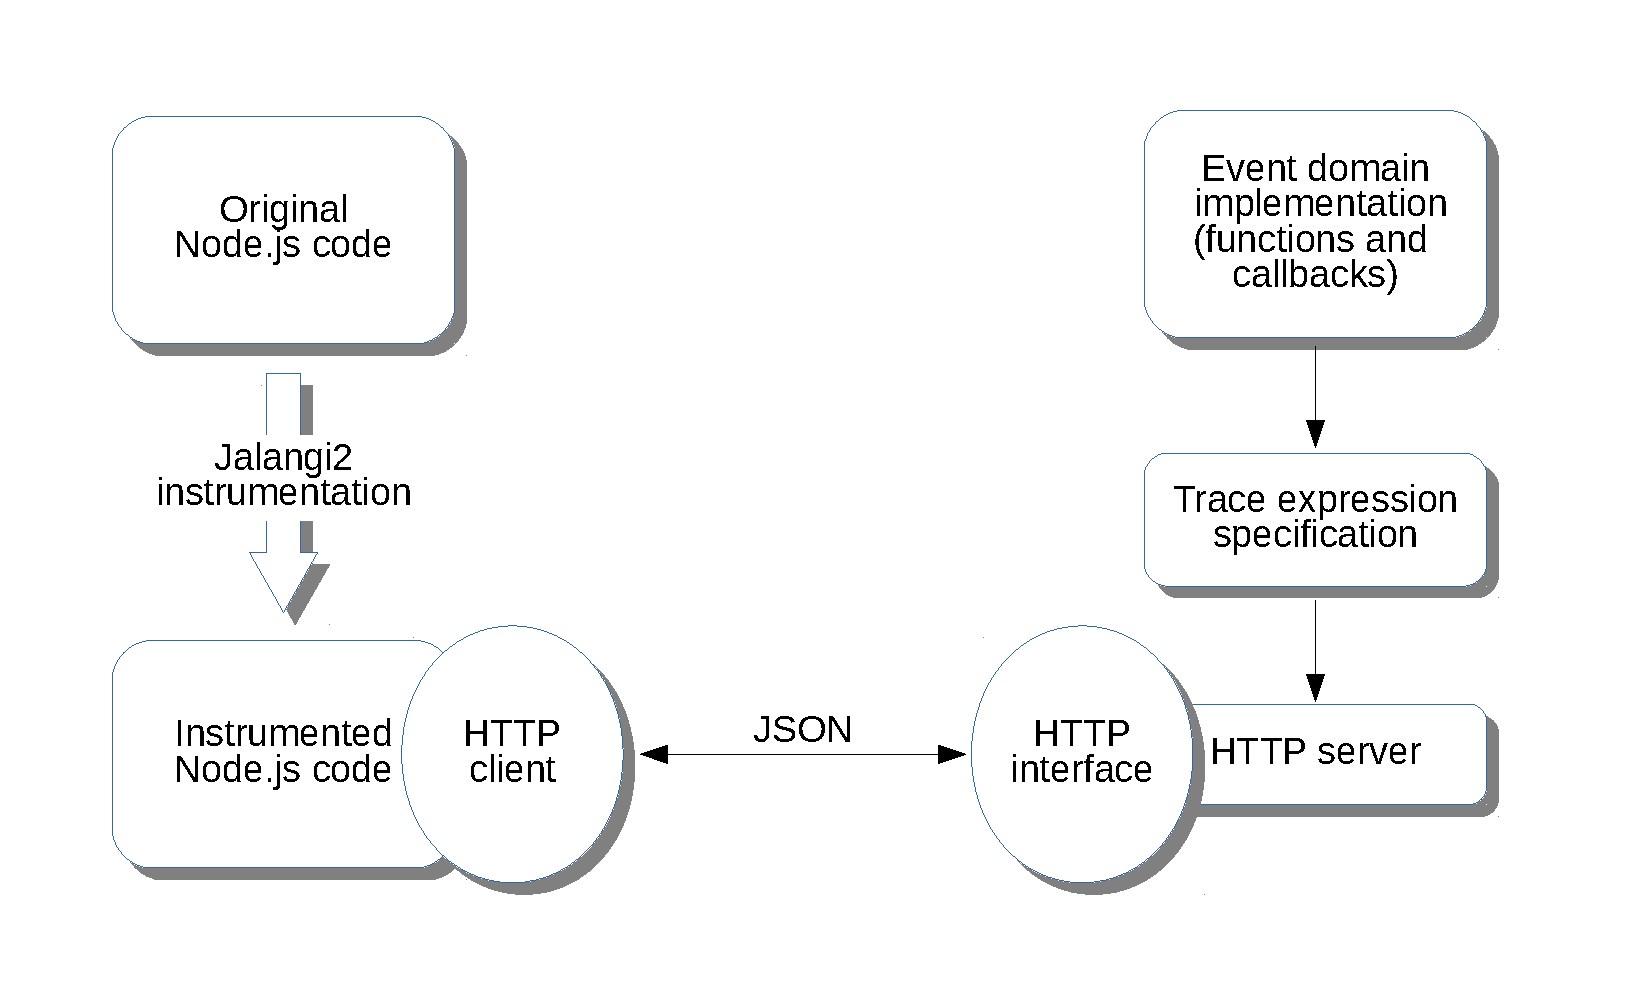
\includegraphics[width=.8\textwidth]{fig/architecture}
\caption{Monitoring architecture for Node.js exploiting SWI-Prolog server with an HTTP interface.}
\label{fig:arch}
\end{figure}

The component on the left-hand-side has been developed in JavaScript and is responsible for emitting through \emph{code instrumentation} all relevant events that have to be monitored
at runtime, while the other on the right-hand-side consists of an HTTP server, written in SWI-Prolog, which receives from the instrumented code all monitored events in form of HTTP requests in JSON format, and checks them against a specification consisting of Prolog components defining the used event domain and trace expression; in case the server detects an error because the received event does not meet the specification, it sends back details about the failure in response to the client. Implementation through an HTTP server allows decoupling of the monitored system from the monitor, and
favor interoperability, and runtime verification of distributed systems.

%% Further details on the approach and the implementation with Jalangi2 can be found in the related paper \cite{TowardsIoT17}.

%% The core idea is to modify the original source code of the program to be monitored in a way that allows observation of relevant events.
%% Once an event is observed, the monitor can verify it against the specification, eventually acting in case of erroneous behavior.

\subsection*{Instrumentation}
We have employed \emph{Jalangi2} \cite{jalangi}, a mature tool supporting instrumentation with 
% gia' linkato nelle prime pagine
%\footnote{\url{https://github.com/Samsung/jalangi2}} \cite{jalangi}
arbitrary code which can be inserted right before or after any main JavaScript operation: access to properties, declarations, functions and methods invocation, among others. Jalangi2 also gives access to information about the operation itself, as the arguments of a function call or the target object of a property access.
The tool allows for state-of-the-art performance in the context of code instrumentation for dynamic analysis.
To the best of our knowledge, the most similar tool is Linvail \cite{linvail}, though its performance are reported to be worst by an order of magnitude (w.r.t.\ the overhead).

Despite the flexibility of Jalangi2, instrumenting code to determine when asynchronous calls and their callbacks are executed and to send the corresponding events in form of an HTTP request was a challenging task, that required to develop more than 450 SLOC of non trivial JavaScript code, to tackle
several issues, among which the following ones are the most significant:

\begin{itemize}
\item Anonymous and arrow functions are extremely common in JavaScript and Node.js applications, and the information about their name
  provided by Jalangi2 for function calls is completely  useless, hence we had to implement from scratch a reliable mechanism to identify them.
\item Jalangi2 does not provide any mechanism for coupling asynchronous function calls with their callbacks, a feature which is
  necessary to allow RV to detect undesired non-deterministic behavior due to the invalid use of asynchronous operations, as shown in
  \Cref{sec:examples}. %% the same asynchronous function can be used multiple times with different arguments and callbacks, and vice versa.
To this aim, the instrumentation we have implemented dynamically wraps callbacks \emph{at runtime} and generate a unique identifier for each one of them.
\item Jalangi2 allows insertion of instrumented code for function calls at four different sites: before and after a function call (caller sites), 
  before the execution of a function body starts, and after the execution of a function body completes (callee sites). Since
  events are tracked through code instrumentation, all four kinds of sites are useful for library functions that cannot be
  instrumented (either because they are not implemented in JavaScript, or because instrumentation would imply a severe performance penalty):  the caller sites
  are used when calls to library functions have to be monitored, while the callee sites are useful to track calls to callbacks that are passed to
  library functions.

  This flexibility comes at a cost when monitoring functions whose source code is available because they are part of the very same program under analysis; in this case two duplicate events would be generated as HTTP client requests sent to the monitoring Prolog server. To this aim,
  the instrumentation we have implemented keeps track of all kinds of function calls, to avoid such duplications.
  
\item In case of method calls, it is useful to identify the target object on which the method has been called, to keep track of the correct
  flow of methods that can be safely invoked on a specific object; Jalangi2 solves this problem only partially,
  because it exposes  the target objects of method calls as mere JavaScript values, without information on the identity of the objects.
  Since the information carried by events are converted into JSON format before sending them to the monitoring server, the identity of objects are lost 
  in such a conversion. Our implementation uses a weak map to keep track of object identities and to generate events containing a unique identifier
  for target objects of method calls; a weak map is employed to avoid issues with garbage collection.

\item Though JSON is a natural fit for JavaScript objects serialization, some important aspects needed to be handled.
Objects containing circular references, for instance, are quite common in Node.js modules, but they cannot be encoded in JSON, and the JavaScript standard library serialization (\lstinline|JSON.stringify|) throws an error on such objects.
Furthermore, JavaScript supports getters, which are special functions invoked when a property is accessed.
During experiments with the \lstinline{http} module, we found that some modules add getter functions to objects before their code can actually be
correctly executed; unfortunately, the standard serialization offered by \lstinline|JSON.stringify| invokes getters during stringification, hence
JSON conversion  breaks if an object contains a getter performing some illegal operation. 
For these reasons, we have  adapted the JSON serialization process by providing a suitable replacer\footnote{See the code at \url{https://github.com/LucaFranceschini/trace-expressions/blob/master/jalangi/stringify-trunc.js}} able to correctly deal
with cyclic objects and getters.

\item Another challenge consists in efficient handling of HTTP requests that have to be sent to the 
  monitoring server. Module \lstinline{http} of Node.js offers a quite simple interface for that, through the  function
  \lstinline{http.request} which is able to send requests in a quite efficient way. To ensure good performances, such an operation is
  asynchronous, hence, as shown in \Cref{sec:examples}, it does not guarantee that events sent in form of http requests are delivered in the  
  desired order, unless a proper callback is employed; however, ensuring that events are sent in the correct order is important to guarantee correctness of RV. As a preliminary solution, we have conducted some experiments with the
  synchronous version of \lstinline{http.request} provided by \lstinline{npm}; unfortunately, we have discovered that with such a solution
  the file explorer server employed in our benchmarks (see Section~\ref{sec:exps}) could serve no more than
  three requests per second when monitored. That was an unacceptable result even when limiting RV to the development stage
  for debugging and testing purposes.

  To solve such a problem, the instrumented code creates a child process with \lstinline{child_process.fork} and
  sends the detected events to it through the established IPC channel, by calling the synchronous function \lstinline{subprocess.send};
  the child process sends all received events to the monitoring server by using the \lstinline{http.request} function and by guaranteeing
  that requests are issued in the desired deterministic order, by passing to \lstinline{http.request} a proper callback.
\end{itemize}

%% Note that even if we strongly rely on Jalangi2, these issues need to be faced with any code instrumentation framework when applied to Node.js code, because of the very nature of the framework and of JavaScript itself.

%% Our prototype implementation enriches the capabilities of Jalangi by supporting these additional features for Node.js monitoring.
%% We are currently looking at proxy-based alternative approaches based on reflection rather than instrumentation, since proxies \cite{proxy} are now natively supported by JavaScript.

\subsection*{Monitoring server}

The monitoring server is implemented in SWI-Prolog and depends on a Prolog module responsible for
the semantics of trace expressions.

The logic programming paradigm is well suited for the implementation of inference systems, since inference rules can be translated
almost directly to logic clauses.
Furthermore, SWI-Prolog offers native support to cyclic terms (a.k.a. regular terms \cite{Courcelle83}) by preventing occurs check during unification;
in this way, recursive trace expressions can be directly encoded with cyclic terms without introducing an explicit construct to deal with recursive
definitions.
Cyclic  terms can be suitably manipulated with the \lstinline{coinduction}\footnote{\url{http://www.swi-prolog.org/pldoc/doc/_SWI_/library/coinduction.pl}.}
module, provided by the SWI-Prolog library to allow simpler definitions of predicates defined on cyclic terms;
such a module employs a cycle detection mechanism which avoids solving a goal which unifies with a goal that has been previously solved
for the same derivation. In this way, predicates on cyclic terms can be defined coinductively and goals with coinductive predicates
can be solved without infinite loops. The  \lstinline{coinduction} module provides an implementation for
coinductive logic programming \cite{colp}.

%% Another useful optimization consisted in reducing the network traffic 
%% between the monitored application and the monitor; while
%% the first version of the instrumentation was designed to send
%% all detected events, the optimization version sends only those events 
%% which are relevant for the verification.

%% This work is a preliminary step towards runtime verification of Internet of Things applications,
%% both because Node.js is emerging as a standard framework for IoT development, and the implementation through an HTTP
%% server offers a natural support to verification of distributed systems, where (instrumented) devices can send events to a monitoring server.



\section{Experiments}
\label{sec:exps}

In this section we report on the experiments conducted with the prototype tool
whose implementation has been described in \Cref{sec:impl}. All code required for reproducing such experiments are available
at \url{https://github.com/LucaFranceschini/trace-expressions}. %%%\url{http://www.disi.unige.it/person/AnconaD/\toolName}.

Since one of the main use of Node.js is the development of Web applications,
we have focused on runtime verification of code based on the \lstinline{http} module.

First, the documentation of the module\footnote{Available at \url{https://nodejs.org/api/http.html}.} has been inspected with the purpose of mining specifications of the features provided by \lstinline{http}.
Several of them can be easily translated in corresponding trace expressions
that have been employed in our tool to automatically monitor correct use of the \lstinline{http}
module by client code.

Six constraints that are not enforced by the library have been identified on the use of the functions exported by \lstinline{http};
correspondingly, six trace expressions have been derived to
dynamically check such constraints and detect the related bugs.
In each trace expression we use the filter operator to restrict the event domain to functions that are relevant for the specification.

The tool has been tested in two different ways.
At a first stage, simple server and client Node.js applications based on \lstinline{http} have been developed,
and violations of the module specifications have been deliberately introduced in the code,
to verify that the tool is effectively able to detect illegal use of the \lstinline{http} features.

Then, at a second stage, the tool has been experimented with real and widely used code based on  \lstinline{http}.
To this aim, the Web application framework Express\footnote{See \url{https://expressjs.com/}.} has been
selected for our test: it offers a large number of HTTP utility methods and middleware functions for more rapid, efficient
and robust development of HTTP APIs, and, for these reasons, several popular Node.js frameworks and Node.js Web applications
are built on top of it.

\subsection{Mining Specifications from the \lstinline{http} Module Documentation}\label{sec:spec-minining}

The documentation of the standard Node.js \lstinline{http} module has been carefully inspected to find illegal uses
of the provided features.
As an example, \Cref{fig:httpDoc} shows an excerpt concerning \lstinline{http.ClientRequest};
objects are internally created with this constructor and returned from \lstinline{http.request()}.
\begin{figure}
	\framebox{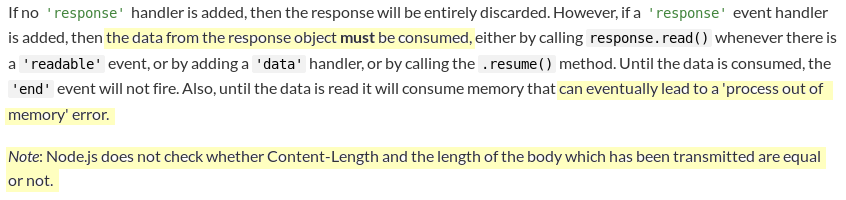
\includegraphics[width=\textwidth]{fig/httpExcerptHighlight}}
	\caption{Excerpt from the \lstinline{http} documentation at \url{https://nodejs.org/api/http.html}.}
	\label{fig:httpDoc}
\end{figure}
The highlighted sentences reveal two possible issues:
\begin{itemize}
	\item \textbf{unconsumed data}: in case the client defines a handler for the server response, data from the response must be actually consumed (through \lstinline|res.on('data', ...)|), otherwise a memory leak will occur;
	\begin{lstlisting}[language=javascript]
const req = http.request(options, res => {
	// BUG! no data read, and 'end' will never happen
	// res.on('data', chunk => {...});
	res.on('end', () => console.log('response received'));
});
req.end();
	\end{lstlisting}
	\item \textbf{content length}: unchecked length of the body of a request/response can block the communication, or data can be lost, as already shown in \Cref{sec:web-req}.
\end{itemize}
In the first case, the correct behavior can be captured by the following trace expression $\tau$ defined as follows (\(\eventSet\) is the event domain in use):
\begin{align*}
	\eventSet &= \bigcup_{
			\substack{
				\mathit{obj} \in \mathbb{N}\\
				\mathit{label} \in \{ \mathit{data}, \mathit{end} \}
			}
		}
		\{ \ont(\mathit{obj}, \mathit{label}) \} \\
	\tau &= \var{res}{\ont(\avar{res}, \mathit{data}) \prefixop ((\ont(\avar{res}, \mathit{end}) \prefixop \emptyseq) \shuffleop \tau)}
\end{align*}

Variable \(\avar{res}\) corresponds to the identifier of the specific response, whereas event type \(\ont\) capture the handling of events \lstinline{'data'} and \lstinline{'end'}, as shown in the code above.
Like in previous examples, combination of shuffle and recursion is essential to be able to deal with an arbitrary number of different responses which can be received by a client.

In the second case, the trace expression which is used for checking the correct behavior of code dealing with
\lstinline{http.ClientRequest} objects has already been presented in \Cref{sec:web-req}.

Besides the two properties discussed above, the following four additional specifications have been mined from
the documentation and expressed with corresponding trace expressions:
\begin{itemize}
	\item \textbf{omitted body}: depending on the request received by the client or the response sent by the server, there are cases when the HTTP message must not contain a body, hence a server which tries to include a body in such situations does not behave correctly. The different cases require different treatments and trace expressions, as follows:
	\begin{itemize}
	  \item \textbf{HEAD request}. The method of the request sent by the client is HEAD:
		\begin{lstlisting}[belowskip=-3em]
const req = http.request('www.example.com', {method: 'HEAD'});
// BUG! body is ignored in HEAD requests
req.write('some content');
req.end('some more');
		\end{lstlisting}
		For every HEAD request, method \lstinline|write| should never be called and \lstinline|end| should only be invoked with no content to be sent:
		\begin{align*}
			\eventSet &= \bigcup_{\substack{\id \in \mathbb{N} \\ \avar{bytes} \in \mathbb{N}}}
			\{ \req(\id), \writet(\id, \avar{bytes}), \myend(\id, \avar{bytes}) \} \\
			\tau &= \var{\id}{\req(\id) \prefixop ((\myend(\id, 0) \prefixop \epsilon) \shuffleop \tau)}
		\end{align*}
		\item \textbf{204 response}. The response of the server has status code 204:
		\begin{lstlisting}[belowskip=-3em]
const server = http.createServer((req, res) => {
	res.writeHead(204);
	// BUG! 204 responses should include no body
	res.write('hello');
	res.end('end');
});
		\end{lstlisting}
		Whenever a 204 status code is set for a response, no content is expected; however, if the status code is set to a different value, the specification allows to send data:
		\begin{align*}
			\tau &= \var{\avar{cb}}{\mathit{createServer}(\avar{cb}) \prefixop \tau_{\mathit{cb}}}\\
			\tau_{\mathit{cb}} &= \var{ \avar{res} }{ \cbt(\avar{cb}, \avar{res}) \prefixop (\tau_{\mathit{res}} \shuffleop \tau_{\mathit{cb}}) }\\
			\tau_{\mathit{res}} &= (\mathit{writeHead}(\avar{res}, 204) \prefixop \myend(\avar{res}, 0) \prefixop \epsilon) \orop (\mathit{writeHeadNot}(\avar{res}, 204) \prefixop \tau_w) \orop \tau_w\\
			\tau_w &= (\writet(\avar{res}) \prefixop \tau_w) \orop \var{n}{\myend(\avar{res}, \avar{n}) \prefixop \epsilon}
%			\tau &= \var{id}{\mathit{createServer}(\id) \prefixop \tau'}\\
%			\tau' &= (\writet \prefixop \tau'') \orop (\myend \prefixop \tau') \orop (\mathit{writeHead204} \prefixop \tau''') \orop (\mathit{writeHeadNo204} \prefixop \tau'')\\
%			\tau'' &= (\writet \prefixop \tau'') \orop (\myend \prefixop \tau') \orop (\mathit{writeHeadNo204} \prefixop \tau'')\\
% 			\tau''' &= \mathit{endNoBody} \prefixop \tau'
		\end{align*}
		The event type \(\mathit{writeHead}\) (\(\mathit{writeHeadNot}\)) ensures the given code has (not) been set for the response.
	  \item \textbf{304 response}.
		The method of the request sent by the client is a conditional GET and access is allowed, and the response server has status code 304 (not modified) because the requested document has not been modified.
		The specification for this use case is entirely similar to the previous one, only the status code needs to be changed.
	\end{itemize}
	\item \textbf{Write head}: the method \lstinline{writeHead} allows to add an header to a server response.
	It must only be called once on a message and it must happen before the method \lstinline{end} is called in order to signal to the server that the response is complete.
	If this rule is not followed, then a default header, possibly different from the intended one, is used in the response.
	\begin{align*}
		\tau &= \var{\avar{cb}}{\mathit{createServer}(\avar{cb}) \prefixop \tau_{\mathit{cb}}}\\
		\tau_{\mathit{cb}} &= \var{ \avar{res} }{ \cbt(\avar{cb}, \avar{res}) \prefixop (\tau_{\mathit{res}} \shuffleop \tau_{\mathit{cb}}) }\\
		\tau_{\mathit{res}} &= \var{s}{\mathit{writeHead}(\avar{res}, \avar{s}) \prefixop \tau_{\mathit{end}}} \orop \tau_{\mathit{end}}\\
		\tau_{\mathit{end}} &= \myend(\avar{res}) \prefixop \epsilon
	\end{align*}
\end{itemize}
While some of the mined specifications directly depend from the specific implementation of \lstinline{http}, others
are more related to the specification of the HTTP protocol; indeed, other trace expressions could be mined by looking at the
standard specification of HTTP, to dynamically check that a server (resp. client) implementation in Node.js verifies the HTTP
requirements.

\subsection{Testing the Tool with Simple Applications}
\label{sec:simple-test}
The tool has been tested with the trace expressions of the specifications presented in the previous section by performing
runtime verification of simple servers/clients implemented in Node.js.
For all specifications both correct and incorrect code has been developed, to verify the absence of both false negatives and positives.

Consider for instance the last specification presented in \Cref{sec:spec-minining}:
the header of a server response must be written before calling the \lstinline{end} method which finalizes the response.

A very simple server verifying the specification is the following one:
\begin{lstlisting}
const http = require('http');
const server = http.createServer((req, res) => {
	res.writeHead(200); // preparing response...
	res.end(() => console.log('response sent'));
});
server.listen(80);
\end{lstlisting}

As expected, in this case the tool does not report any anomalous behavior.
However, if we modify the code above as follows
\begin{lstlisting}
const http = require('http');
const server = http.createServer((req, res) => {;
	res.end(() => console.log('response sent'));
	res.writeHead(204); // BUG! writing header after calling end() method
});
server.listen(80);
\end{lstlisting}
and monitor the server with our tool, then we get an error message associated with the following event, corresponding
to a call to \lstinline{writeHead}:
\begin{lstlisting}
{ event: 'func_pre', name: 'writeHead', id: 12, res: undefined, args: [ 204 ], targetId: 10, resultId: undefined }
\end{lstlisting}

Similar examples have been used to test our tool with the other specifications.

\subsection{Testing the Tool with Express}\label{sec:express}

After the simple experiments conducted in the first phase as described in the previous section,
a natural next step towards the assessment of our tool consisted in testing popular real Node.js code
based on \lstinline{http}.
% to do that, we have considered Express\footnote{See \url{https://expressjs.com/}.}, a very (if not the most) popular framework based on \lstinline{http} to develop Node.js web applications.

To this aim, the three components of Express depending on \lstinline{http} (\lstinline{application.js}, \lstinline{request.js} and
\lstinline{response.js}) have been instrumented with Jalangi2, for a total of almost 1K SLOC.
As for the other tests of \Cref{sec:simple-test}, we have reused the same Jalangi2 instrumentation and trace expressions defined in \Cref{sec:spec-minining}.

Then the use of \lstinline{http} by Express has been dynamically monitored with our tool through simple
examples of server applications written with Express as the following one:
\begin{lstlisting}
const express = require('express');
const morgan = require('morgan');
const responseTime = require('response-time');
const serveIndex = require('serve-index');
const path = process.cwd();
const app = express();
app.use(morgan('combined'));
app.use(responseTime());
app.use('/', express.static(path), serveIndex(path, {'icons': true}));
app.get('/*', (req, res) => {
    res.writeHead(404, {'Content-Type': 'text/html'});
    res.end('Not found\n');
});
app.listen(80);
\end{lstlisting}
Although the application contains only a dozen of source lines of code, the
functionalities of the server are not so trivial, thanks to Express and the
associated middleware \lstinline{morgan}, \lstinline{response-time}, \lstinline{serve-static} and
\lstinline{serve-index}.

The \lstinline{morgan} module creates a logger middleware function that allows the server to log (on the standard output, in this example)
information about the received requests, while the \lstinline{response-time} module
creates a middleware that records the response time of the HTTP server, that is, the elapsed time from when a
request enters the middleware to when the headers are written out to the client.

The  \lstinline{serve-static} middleware serves files from within a given root directory (in this case, the same directory
from which the server has been launched), while \lstinline{serve-index} serves an index (with displayed icons in this case)
of the directory of the server based off the URL value of the request. In practice, the server allows inspection of the directory
from which it has been launched, included all its subdirectories, and downloading of all files rooted at it.

Finally, the last call \lstinline{app.get} deals with the case when no directory or file could be found.
The tool has been tested with the server above, and a Node.js client sending requests with random  paths based on its root directory at the frequency of three requests per second.
The tool was able to monitor all relevant \lstinline{http} events triggered in the above mentioned Express components used through the server, showing that our instrumentation and monitoring system can deal with code bases of considerable size using all the main features of the programming language.
For this specific example, no violations of the previously described constraints on the use of the \lstinline{http} module were detected by the monitor.

\subsection{Benchmarks}

All tests presented in Section~\ref{sec:spec-minining} have been employed as benchmarks for performance evaluation
of our prototype on an Intel(R) Core(TM) i7-6500U CPU at 2.50GHz with a 16GB RAM, running SWI-Prolog 7.2.3 on
Linux kernel 4.14.40.
In particular, we have measured how much the performances of all implemented servers are affected by runtime monitoring;
only correct implementations have been considered, to be able to overload servers with arbitrary numbers of requests.
The benchmarks have shown that the overhead of runtime verification is mainly due to code instrumentation, rather than the particular monitored
specification, therefore all measurements have been conducted while verifying the same trace expression, namely, 
the one corresponding to the specification \textbf{omitted body (204 response)}.

Table~\ref{table} shows the results of our experiments. 
\begin{table}[ht]
  \begin{tabular}{|l|l|l|l|}
    \hline
    \textbf{Benchmark} & 
    \textbf{Original} &
    \textbf{Monitored} &
    \textbf{Overhead} \\
    \hline
    \multicolumn{4}{|c|}{HTTP module}\\
    \hline
    Content length & 
    591 RPS &
    528 RPS &
    12 \% \\

    Omitted body (HEAD request)&
    631 RPS &
    588 RSP &
    7 \% \\

    Omitted body (204 response)&
    638 RPS &
    626 RSP &
    2 \% \\

    Omitted body (304 response)&
    634 RPS &
    626 RSP &
    1 \% \\

    Unconsumed data &
    643 RPS &
    739 RPS &
    -13 \% \\

    Write head &
    627 RPS &
    580 RPS &
    8 \% \\
    \hline

    \multicolumn{4}{|c|}{Express}\\
    \hline
    Hello world & 
    766 RPS &
    716 RPS &
    7 \% \\

    File explorer &
    588 RPS &
    312 RPS &
    88 \%\\

    \hline
  \end{tabular}
  \caption{Benchmark results}
  \label{table}
\end{table}
For each benchmark we have measured the average number of served requests per second (RPS) 
with a client running a loop to continuously send requests to the server without waiting to collect its response;
all measurements have been obtained as the average over ten different runs, each consisting
of 100K requests sent to the server.

The second column (Original) displays the values concerning the original server, while the third one
(Monitored) reports the measurements for the same server under monitoring.
For all simple servers directly implemented with the \lstinline{http} module we registered modest overheads, as well
as for the Express server sending the response \lstinline{'Hello world'} to all requests.
Interestingly, the monitored version of \textbf{unconsumed data} outperforms the original version; we have
not investigated yet the reasons of such a behavior.

For the file explorer built with Express and presented in Section~\ref{sec:express}, the client keeps sending GET requests
with randomly generated paths; in this case the overhead is more significant, but still the overall performance 
is acceptable: the server could operate at the rate of more than 300 RPS, while the system had to monitor more than 1.5 million events.
Such a result shows that the optimizations introduced in our prototype implementation allowed us
to get a 100x speed boost, and that runtime monitoring can be effectively employed for testing servers implemented with Express.



\section{Conclusion}
\label{sec:conclu}

We have presented the implementation of a prototype tool able to support
parametric runtime verification of Node.js applications in a distributed environment.

The tool is based on parametric trace expressions, and exploits Jalangi2 for tracing events via code instrumentation, and SWI-Prolog to
implement trace expressions.

Experiments have been conducted on \lstinline{http}, one of the most popular standard Node.js modules,
by mining from its documentation several specifications later expressed with trace expressions.

The mined specifications have been dynamically verified with the tool on several simple examples of HTTP servers and clients,
and with more interesting examples based on Express; these last tests required code instrumentation of the Express components
built on top \lstinline{http} for a total of almost 1K of SLOC, and have shown that the prototype tool is able to support
runtime verification of real Node.js code; the benchmarks show that the implemented optmizations allow a 120x speed boost for the more
complex Express example.
To our knowledge, no other currently available tool allows parametric runtime verification of Node.js applications in a distributed environment.

Although the reported experiments are promising, a considerable amount of work is still required for making our research prototype a tool usable in practice.

\subsection{Experiments}
Runtime verification of Express servers is an interesting result for the tool; unfortunately,
no benchmarking suites are available for further testing our tool, hence we are
considering to include in our suite other Express servers, either implemented by ourselves,
or freely available on the Web.

On the side of specification mining, there are still other interesting properties that can be expressed an dynamically
verified with parametric trace expressions which we are considering to mine both from the documentation of Node.js
\lstinline{http} module, and from the specification of HTTP. Furthermore, there is a number of other widely used Node.js
modules and frameworks as \lstinline{async} and \lstinline{jquery} for which specification mining and runtime
verification would be quite useful.

%% \subsection{Performance}
%% At the moment we have not focused on performance issues, because our first target was to have a proof of concept
%% that it is possible to implement a tool for parametric runtime verification for Node.js applications in a distributed environment.
%% As long as monitoring is used for software verification before deployment, problems with performance degradation are less 
%% stringent; however, the current implementation of our prototype still requires several optimizations to support runtime verification
%% in practice.

%% A first practical way to obtain a speed up of the monitored application is to
%% allow asynchronous communication between the instrumented code and the monitor;
%% indeed, the current implementation is based on synchronous communication, because this is
%% a simple way to guarantee that the monitor always receives events in the correct order.
%% Asynchronous communication is more complex to implement and can be achieved in different ways;
%% anyway, the speed up obtained by this solution depends on the responsiveness of the monitoring server,
%% which cannot be easily estimated without experimental data, because it depends on the specifically employed trace expression
%% for runtime verification.

%% Another useful optimization consists in reducing the network traffic 
%% between the monitored application and the monitor.
%% This can be effectively achieved in the following ways.

%% The current instrumentation implemented with Jalangi2 sends to the monitor
%% all events of the domain; in our case, all calls and returns from functions/callbacks.
%% However, the instrumentation can be configured so that it sends only those events 
%% of the domain which are relevant for the verification.

%% We have discussed in \Cref{sec:impl} that problems with getters and circular objects
%% prevented us to use \lstinline{JSON.stringify} to serialize values of the events to be sent to the
%% monitor. The customized version of \lstinline{stringify} we have implemented for the tool
%% can be optimized in several ways at the cost of a more complex code; for instance,
%% objects are always serialized at arbitrary depth (up to circularity, of course), but for
%% all kinds of verifications we have tested with our experiments, it is sufficient to serialize objects
%% at fixed depth not larger than 4 levels.

%% Finally, to optimize connection time, it would be worth sending sequence of events rather than one
%% event at time as happens in the current implementation.

\subsection{Error Reporting and IDE}
So far error reporting has been neglected, and in case of failure the only available information
regards the unexpected event that has been traced; clearly, more informative error messages
are required to allow the user to understand and locate more easily the detected problem.

Jalangi2 already supports information about the location of the original code that has been
instrumented, hence it should not be difficult to display the line of code and name of the file where
the faulty event has originated.

For error messaging, the SWI-Prolog implementation already supports identification of
all trace expressions that constitute a certain specification, hence associating specific error messages with them
would be a simple extension.
Moreover, the trace expression specification could be serialized and sent to the program for reporting purposes.
To this aim, JSON Schema \cite{jsonschema} can be useful.

Finally, at the moment, trace expressions must be written directly in Prolog and, although the used syntax
is similar to that defined in the paper, the interpreter adopts non standard rules to manage operator precedences,
and does not statically detect ill-formed trace expressions.

To this aim, we are developing in \textit{Xtext}\footnote{\url{https://eclipse.org/Xtext/}} an IDE
to write specifications with trace expressions at a higher level, and to automatically generate
the corresponding Prolog code. \textit{Xtext} allows such an IDE to be integrated as an Eclipse plugin
with support for syntax-highlighting, auto-completion,
and a number of static checks useful for early error detection of the written specification.


\printbibliography
%%\bibliography{main}

\end{document}

